\documentclass[11pt]{article}
\usepackage{graphicx}
\usepackage[pdf]{pstricks}
%\usepackage{mathtools}
\usepackage{amssymb,amsmath}
\usepackage{textcomp}
\DeclareMathOperator*{\argmin}{arg\,min}

%\usepackage{subcaption}
%\usepackage{float}
\usepackage{setspace}
\usepackage{fullpage}
\usepackage[font=scriptsize]{caption}
%\usepackage{fullpage}
%\setcounter{secnumdepth}{1}
\begin{document}

\title{Fused regression for network inference in multiple species}
\author{Kari Y. Lam, Zachary M. Westrick, Christian L. M\"{u}ller, Lionel Christiaen, Richard Bonneau}
\maketitle

\begin{abstract}
Learning gene regulatory networks is essential to our understanding of cell behavior and response to external stimuli. Methods for network inference from large datasets have been developed and used for a wide variety of species; however, these approaches consider the problem as independent in each species even though there is known to be conservation of gene regulation even in distantly related species. We introduce a method that allows data to be pooled across species in a principled way based on gene orthology and demonstrate that it improves network inference even when the orthology is incomplete. We further refine this method with an algorithm that attempts to learn the true conserved subnetwork from a larger set of potentially conserved interactions. 
\end{abstract}

\section{Introduction}
As the volume and variety of genome scale data have exploded, the goal of accurately modeling gene regulatory networks has become more attainable. Large-scale data collection efforts have contributed to the development of high quality networks, but there remain many biological processes and organisms for which there does not exist enough data. Furthermore, as new technologies are developed and some old ones are replaced, such as RNAseq and microarray, it becomes important to be able to combine different data sets, lest we lose valuable information from previous studies. The problems of inferring networks in related species, processes, and using different technologies likely are not independent ones, and benefit from the infusion of additional data.

The extent to which datasets are related is an important consideration when deciding to combine them. Abundant data in one species should be a useful source when learning the network of a related species. But often, how much and what of orthologous networks' structure is conserved, is not known a priori. We would like, then to be able to learn the conserved subnetwork in order to make better predictions using multi-source network inference. 

We present two methods for network inference which use fused regression, a type of penalized least squares regression, in which the difference of regulatory weights which are thought to be similar are penalized. Our fused L2 method uses a ridge fusion penalty on these differences, and is useful where the relationships between nodes (similarity of genes between data sets) is reliable. Our adaptive fusion uses a non-concave saturating fusion penalty to simultaneously learn multiple networks and conservation of these networks. 

To learn gene regulatory networks, we employ a linear model of gene expression in which the rate of expression is assumed to be proportional to a weighted sum of transcription factor expression. These weights represent the regulatory interactions we wish to learn. We can fit these weights simultaneously in multiple data sources of interest using time series and steady state expression data. This is similar to many existing network inference methods and produces identical answers to fitting each network separately. To take advantage of cross-dataset information, we introduce additional constraints on the problem that penalize differences between regulatory weights which are expected to be similar. Genes are not always regulated by the same transcription factors under different conditions. For example, a TF which promotes expression of a gene under a given process may repress that same gene at another point. Using data from these conditions to learn one network will prevent the identification of these contradictory regulatory interactions; it is therefore important to be able to combine data in a principled manner. We can use knowledge about the conservation of regulation while leveraging the additional data to learn networks describing disparate processes. In the case of multiple species, there has been a great deal of work showing that functional conservation exists in gene regulatory networks even across large evolutionary distance. We make the assumption that if a transcription factor in one species is orthologous to a TF in a related species, and a gene in the first species is orthologous to a gene in the second, then the interaction between the TF and gene in the first species should be similar to the interaction between the orthologous TF, gene pair in the second species. By utilizing information about conservation of gene function across data set, species, and biological process, we enable the usage of less directly relevant data and improve network inference.

There exist several tools for identifying orthologous genes using sequence similarity. Although sequence similarity is a useful predictor of functional similarity, we recognize that some genes have taken on different functions and therefore may have new regulatory interactions. When this occurs, the benefits in overall performance from our L2 fusion approach come at the cost of impaired prediction of regulators for these genes. The constraints we impose favor weight configurations in which fused interaction weights are similar to one another. Our fused L2 method minimizes a cost function that strives to simultaneously fit expression data in each species and produce networks that are consistent with these evolutionary constraints. When a gene's regulators have changed through evolution, there may be no way of achieving both these goals. Similarly, if a gene has different regulators during different processes, the expression data may conflict with the fusion constraints. In these cases, the network inference procedure would be improved by relaxing or ignoring these evolutionary constraints. However, we don't know a priori which constraints to enforce and which to relax.  

We approach this problem by introducing a saturating penalty function based on work in statistics to develop unbiased regularization penalties for regression. The resulting cost function is non-convex and difficult to optimize and fares less well in the underdetermined case; however, we can approximate its solution and obtain deeper insights into functional similarity than is available through orthology or the comparison of separately learned networks. When the quantity of data is sufficient to produce high quality networks, our adaptive fusion approach improves performance of network inference; this is achieved in part through the identification of presumptive orthologs with different functions. In simulated data, when we introduced faulty orthology information, our method not only correctly identified which evolutionary restraints to enforce and which to relax, but also outperformed the control case where no incorrect orthologs were used. 

We test the ability of fused L2 and adaptive fusion to improve network recovery on both synthetic data and Bacillus subtilis and Bacillus anthracis. We explore the circumstances under which each approach is optimal, and evaluate the robustness of adaptive fusion to incorrect orthology, simulating the biologically relevant case of neofunctionalization. 

\section{Methods}
\subsection{Gene regulatory network}
We represent gene regulatory networks as a matrix of weights, where rows index transcription factors and columns index genes. The weight in a given position represents the regulatory weight of that TF on that gene; positive weights represent activation, negative weights represent repression, and 0 weights represent the absence of an interaction. We begin with an existing framework for estimating the interaction weights in a gene regulatory network (GRN). In the Inferelator algorithm, linear differential equations are used to model changes in gene expression. The rate at which the observed mRNA expression of gene $i$, $x_i$, changes is governed by degradation of existing transcripts with rate $\alpha$ plus a linear combination of transcription factor (TF) expressions. 
\begin{equation}
\frac{\mathrm d}{\mathrm d t} x_i = -\alpha_{i}x_{i} + \sum \beta_{i,j}x_{j}
\end{equation}
We are interested in learning $\beta$, the matrix defining the influence of each TF on each gene. We fix the decay rate $\alpha$ for all genes, and set it assuming a time-constant of 10 minutes [CITATIONS], as in [CITATIONS]. Let $x_i(t)$ be the expression of gene $i$ at time $t$. Given time-series data on the expression of gene $i$ at timepoints $t_k$ and $t_{k+1}$, we can approximate the rate of change of $x_i$ as $x_i'(t_k)=\frac{x_i(t_{k+1})-x_i(t_k)}{t_{k+1}-t_k}$. We can treat steady-state data as having a derivative of zero. This gives us, for each gene $i$ and time $t_{k}$ an equation

\begin{equation}
\frac{x_i(t_{k+1})-x_i(t_k)}{t_{k+1}-t_k} + \alpha_{i}x_{i}(t_k)= \sum \beta_{i,j}x_{j}(t_k)
\end{equation}
\noindent We can summarize these equations in matrix form as
\begin{equation}
Y = X \beta 
\end{equation}
\noindent We approach the learning of the $\beta$ matrix using regression. Because there are typically far fewer conditions than possible regressors (TFs), we introduce a ridge regularization constraint with weight $\lambda_R$ and solve
\begin{equation}
\argmin_\beta\vert \vert X\beta - Y_2 \vert \vert ^2 + \lambda_R \vert \vert \beta \vert \vert ^2
\end{equation}
This is essentially the same basic formulation as was used in the Inferelator algorithm, which we extend to the case of simultaneously inferring the GRNs of multiple species. 

\subsection{Fused gene regulatory networks}
We hypothesize that related species should be governed by similar but not necessarily identical gene regulatory networks. We approach the problem of cross-species GRN inference by introducing constraints into the above regression formulation to penalize differences between interaction weights that are expected to be similar based on gene orthology. We can then solve the penalized regression problems simultaneously, in order to obtain a GRN for each species. Consider the case of organisms $A$ and $B$, governed by GRNs $\beta^A$ and $\beta^B$ (the following approach applies equally well to more than two species but for simplicity we continue with the case of two species). If TF $g^A$ in organism $A$ and TF $h^B$ in organism $B$ are orthologs, and gene $k^A$ and $l^B$ are orthologs, then we expect that the $g^A \rightarrow k^A$ interaction weight should be similar to the $h^B \rightarrow l^B$ interaction weight, and we introduce a fusion constraint between these analogous interactions. In terms of the above regression formulation, we expect that $\beta^A_{g,k} \approx \beta^B_{h,l}$, and include a penalty term $p_{\lambda_S}(\beta^A_{g,k} - \beta^B_{h,l})$ to the quantity being minimized in order to ensure similarity. The parameter $\lambda_S$ controls how highly to penalize differences between fused coefficients and controls the tradeoff between fitting the expression data and producing a set of networks that conform to evolutionary constraints. This gives us the final equation to be minimized 
\begin{equation}
\argmin_{(\beta^A, \beta^B)} \displaystyle\sum_{S \in (A, B)} \vert \vert X^S\beta^S - Y^S \vert \vert ^2 + \lambda_R \vert \vert \beta^S \vert \vert ^2 + \displaystyle \sum_{\beta^{S_1}_{g,k} \approx \beta^{S_2}_{h,l}} p_{\lambda_S}(\beta^{S_1}_{g,k} - \beta^{S_2}_{h,l})
\end{equation}

where the second sum is over pairs of interactions with fusion constraints. 

When the penalty $p_{\lambda_S}$ is the L2 norm, the entire problem can be solved through linear regression with a suitable design matrix. The regulators of a pair of genes can be solved independently as long as the pair is not linked by fusion constraints, or a chain of fusion constraints; thus the problem of cross-species GRN inference decomposes into a large number of manageable regression problems as long as the orthology mappings are sparse.


When there is a one-to-one orthology between the species being considered (ie different cell-lines of the same organism), the choice of $\lambda_S$ allows one to interpolate between fitting each network independently ($\lambda_S=0$) and pooling data together as if it came from one source ($\lambda_S=\inf$). Part of the appeal of the approach, however, is that it allows pooling of data even when there is incomplete orthology. By introducing constraints on the similarity of individual interactions, rather than on the networks as a whole [CITE IBM?], we can pool some information across species even when an arbitrarily small fraction of genes have orthologs. This is particularly useful when dealing with a large number of species; pairwise orthologies may be nearly complete even when the number of genes present in every organism is small. 

\subsection{Solving fused L2 problems using augmented matrices}
The problem of solving a multi-valued regression problem can be converted into the problem of solving a single valued regression problem by vectorization.
Specifically, if $Y \in R^{N \times M}$ then we form $A =$ diagonally concatenate $X$, $M$ times (with the remaining entries 0),
$y =$ vertically concatenate the columns of $Y$

$$\underset{w}{min} ||Aw - y||_2^{~2}$$

We can then define $W_{i,j} = \beta_{(j-1) \times N + i, (j-1) \times M + j}$ which is the desired form.
This is equivalent to the original problem due to the block structure of matrix multiplication

Given $X_1... X_S$ matrices, $X_i \in R^{N_i \times K_i}$ we define $N = \sum_{i=0}^S N_i$, $K = \sum_{i=0}^SK_i$ and $X \in R^{N \times K}$ by diagonally concatenating $X_1...X_S$.
In this new matrix, the first $K_1$ features correspond to features of $X_1$, the next $K_2$ features the features of $X_2$ etc.
Similarly, the first $N_1$ samples correspond to samples of $X_1$, the next $N_2$ to $X_2$ etc.
Solving the regression problem associated with each source is equivalent to solving the problem $\underset{W}{argmin}||XW-Y||$ where $Y$ is defined in the same way as $X$.
The weight matrix $W$ has a block diagonal structure:

\begin{figure}[h!]
    \centering
    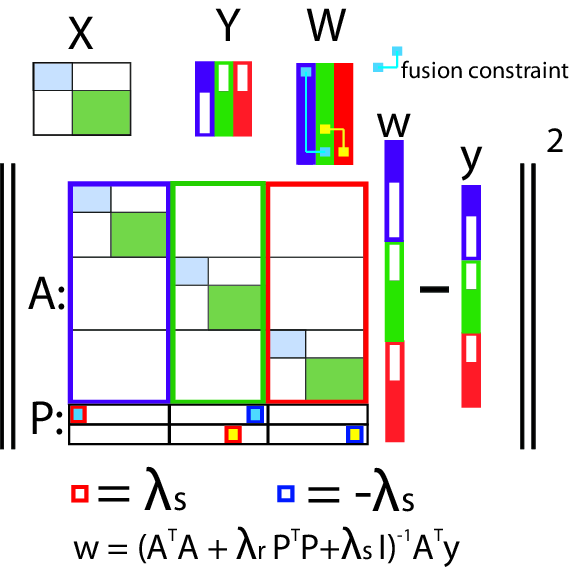
\includegraphics[scale=.5,trim=0mm 0mm 0mm 0mm,clip]{direct_solve.png}
\end{figure}

The fused multi-source regression problem can solved by constructing a multi-source design matrix $X$ and data matrix $Y$, and then vectorizing.
The regression problems associated with two columns $g,h$ of $Y$, where $g$ came from $Y_1$ and $h$ came from $Y_2$, are independent, unless there is a constraint chain of length $L$ with the form (where $x$ is arbitrary)

%$$(G, j_0, g, J_1, j_1, m_1) \rightarrow (J_1, j_1, m_1, J_2, j_2, m_2) \rightarrow (J_2,j_2,m_2,J_3,j_3,_m3)...(J_P, j_P, m_P, H, j_{P+1}, h)$$
$$(Y_1, j_1, g, Y_2, j_2, h) \rightarrow (Y_2, j_2, h, Y_3, j_3, k)$$

where the $j$s refer to transcription factors. In subproblem 1, $j_1$ regulates gene $g$; $j_1$ is orthologous to $j_2$, a transcription factor of subproblem 2, which regulates $h$, a gene which is orthologous to gene $g$. There exists a chain because ($j_1$, $g$) is a TF, gene pair which is fused with ($j_2$, $h$), which is fused to ($j_3$, $k$).
We use depth-first search to identify linked columns of $Y$, and then solve the fused regression problem directly by vectorizing those columns.
In order to incorporate the fusion penalty, we append to the resulting design matrix one row \emph{per connected constraint}, which contains $\lambda_S$ in the column associated with $Y_g,i,j,$ and $-\lambda_S$ to the column associated with $Y_h, i',j'$ for constraint $(Y_g,i,j,Y_h,i',j')$. Call this resulting matrix $X_P$.
The vector $Y$ is augmented by appending an appropriate number of zeros to produce $Y_P$. As a result, each entry in the output of $X_P b$ in the columns associated with each constraint contain $b_{i,j} - b_{i',j'}$.
These entries each contribute  $||b_{i,j} - b_{i',j'}||^{~2}$ to the squared error $||X_Pb - Y_P||_2^{~2}$

In the context of regression for GRN inference with multiple cell sources, each gene $j$ from source $1$ has constraints $\forall_{i \in \{TFs\}} (1, i, j, 2, i’, j’)$ where $i',j'$ are the same gene in a different cell line.
As a result, each gene has only one constraint and the chain has length $L=2$.
%In general, however, solving the fused regression problem directly, even after factoring constraints, involves at least one inversion of an $L\sum_{i=0}^S K_i \times L \sum_{i=0}^S K_i$ matrix, taking $O((L\sum_{i=0}^S K_i)^3)$.
In general, however, solving the fused regression problem directly, even after factoring constraints, involves at least one inversion of an $p\sum_{i=0}^S K_i \times p \sum_{i=0}^S K_i$ matrix where $p$ is the size of a column subset such that there is a constraint chain $L$ linking an element of each column to an element in every other column in that subset, taking $O((p\sum_{i=0}^S K_i)^3)$.
Although the sparse structure of $X_P$ makes this somewhat more tractable, it is still impractical for large $L$.


\subsubsection{Equivalent prior}
Our L2 fusion penalty is equivalent to assuming a Gaussian prior with variance proportional to $\frac{1}{\lambda_S}$ on differences in parameters with fusion constraints. Combined with the regularization constraints, this forms a multivariate Gaussian prior on weights in both networks. When using our method on systems with incomplete orthology mapping, this results in different prior probability distributions for those parameters with fusion constraints and those without. We adjust for this by solving for a constant to multiply fused interactions by to equalize the volumes of the prior distributions. The intent of this adjustment is to ensure that constrained interactions are not on average more highly penalized, which may tend to drive their weight towards zero, causing them to be excluded from the network. 

\subsection{Adaptive fusion}
Fusion constraints are intended to penalize dissimilarity between interactions thought to be evolutionarily analogous. Because fusion constraints are L2, interaction weights which differ from each other by a large amount are excessively penalized, which effectively ensures that fused interactions are assigned similar weights. This may be inappropriate for interactions which are identified based on orthology as being analogous, but which are no longer similar due to evolutionary changes. We propose that a saturating penalty may be useful for dealing with uncertainty about which interactions are conserved. 

With a saturating fusion penalty, fused interactions which appear to be very different based on expression data are allowed to unfuse from one another. A closely related problem has been studied in the context of LASSO regularization, where it was shown by Fan and Li that using a saturating penalty retains many of LASSO's desireable properties while removing its bias towards 0. They further showed that, although the resulting loss-function is nonconvex, good results can be obtained with a local quadratic approximation of gradient descent. Several saturating penalties, such as SCAD [Fan Li 2001] and MCP [Zhang], have been discussed in the context of sparse regression. We introduce a modified form of MCP to the problem of penalizing differences between fused coefficients. The principle difference between the penalty we adopt and SCAD/MCP is that both of these penalties are L1 like at the origin, producing sparse solutions. Because we are penalizing differences in interaction weights, rather than the weights themselves, there's no particular reason to prefer sparsity. 

We use a penalty on the difference between fused coefficients $\theta$ which is L2 like at the origin, begins to level out at $\theta = \frac{a}{2}$, and saturates at $\theta = a$. Written in terms of its derivative, the penalty $p'_{\lambda, a}$

\begin{equation}
p'_{\lambda,a}(\theta) = \left\{
    \begin{array}{lr}
    2\lambda\theta & \text{if } \theta \leq \lambda\\
    \text{max}(\lambda_S(a-\theta),0) & \text{if } \theta > {a \over 2}
    \end{array}
    \right.
\end{equation}

We also implement MCP:

\begin{equation}
p_{\lambda,\gamma}(\theta) = \left\{
    \begin{array}{lr}
    \lambda\theta^2-{ \theta^2 \over 2\gamma} & \text{if } \theta \leq \gamma\lambda\\
    {1 \over 2}\gamma\lambda^2 & \text{if } \theta > \gamma\lambda
    \end{array}
    \right. 
\end{equation}

With derivative

\begin{equation}
p'_{\lambda,\gamma}(\theta) = \left\{
    \begin{array}{lr}
    2\lambda\theta - {\theta \over \gamma} & \text{if } \theta \leq \gamma\lambda\\
    0 & \text{if } \theta > \gamma\lambda
    \end{array}
    \right.
\end{equation}
    
As in [Fan Li], we use solve using iterative local quadratic approximation. 

Specifically, $\beta^S(t)$ is the network on iteration $t$. 

For each fused $B^{S_1}_{g,k} \approx B^{S_2}_{h,l}$ we define:

\begin{equation} 
\theta(0)=0
\end{equation}
\begin{equation}
\theta(t) = \vert B^{S_1}_{g,k} - B^{S_2}_{h,l} \vert
\end{equation}

and introduce a fusion constraint $\lambda = \frac{p'(\theta(t))}{2\theta(t)} $

$\beta^S(t+1)$ is obtained by fitting the ridge-fused model with fusion constraints given by the above $\lambda_S$. This is nice because all our penalties can be treated as L2 and therefore retain the properties of ridge regression. 

\subsection{Model selection}
We can define a leave-out set of priors and choose parameters based on cross-validated AUPR on the leave-out set. 

\subsection{Simulated data}
Generation of simulated data begins with the production of random orthology mappings. We produce a one-to-one orthology by pairing random genes until a specified fraction have been assigned orthologs. This process is carried out separately for TFs and non-TF genes, so that TFs and non-TF genes are never assigned to be orthologous. We then produce a pair of random networks ($B^1$ and $B^2$) as follows. For each unfilled entry in $B^1$ or $B^2$, we enumerate the set $C$ consisting of the entry along with every entry in either matrix to which it is fused. With probability equal to the sparsity rate we assign every entry in $C$ to be 0, otherwise we sample a value $v \sim \mathcal{N}(0,1)$ and independently assign each entry in $C$ to $v + \mathcal{N}(0, \sigma_f^2)$. $\sigma_f$ is a parameter that controls the distribution of differences in the values of fused coefficients, so that the nonzero coefficients of $B^1, B^2$ are distributed as $\mathcal{N}(0, 1 + \sigma_f^2)$.

Given a network $B$, we generate $N$ samples of gene expressions at each of two timepoints. The condition by gene expression matrix for timepoint one, $Y_{T1}$, is sampled randomly from a multivariate Gaussian distribution with identity covariance matrix. $X_{T1}$ is the TF expression sub-matrix of $Y_{T1}$, and consists of columns of $Y_{T1}$ that correspond to TFs. Treating the decay rate as 0, the gene expression matrix at timepoint two, $Y_{T2}$ is sampled as $Y_{T2} = Y_{T1} + BX_{T1}$. This process is carried out separately for each network. 

Following generation of simulated data, we may introduce error into the orthology mapping. This can take the form of discarding a specified fraction of true orthologies (governed by a false-negative rate), or by introducing random false orthologies (governed by a false-positive rate). For convenience, the false-positive rate is specified in units of the number of true orthologs, and not the number of possible orthologs. 

For the purposes of evaluating simulated network recovery, we define a gold standard network as the support of the beta matrices. Priors used in network inference are interactions from the gold standard. The list of priors can be be manipulated to include false positives and false negatives as with the generation of orthologs. 

\subsection{Beta scaling}
In previous work, betas were rescaled as to form a matrix of confidence scores $S$ as follows
\begin{equation}
S_{i,j} = \frac{\sigma^2_{\text{full model for }y_j}}{\sigma^2_{\text{full model for }y_j \text{ without predictor }i}}
\end{equation}
Computing residuals with respect to the data alone would disregard information gained through fusion. Instead, we used an approximation
\begin{equation}
S_{i,j} = \frac{\sigma^2_{\text{full model for }y_j}}{\sigma^2_{\text{full model for }y_j} + B_{i,j}^2 \times var(TF_j)}
\end{equation}
When the residual is uncorrelated with the prediction, then removing regressor $i$ with weight $B_{i,j}^2$ from the model of $j$ will increase the residual by $B_{i,j}^2$ times the variance of regressor $i$. In the case of regularized regression, the regressor and residual need not be uncorrelated, so the approximation will not hold exactly. This scaling is similar to rescaling according to variance explained relative to an augmented design matrix that includes fusion constraints. We use an approximation because it is simpler to compute. The intuition is that a large $B_{i,j}$ may be necessary because TF $i$ varies little across the available data, and these large weights are not suggestive of a true regulatory interaction.

\subsection{Optimization}
We use glmnet to compute the regularization path for the
 ridge penalty. Given a range of $\lambda_R$ values, we fit models for each $\lambda_R$. We use cross validation to select the optimal parameter, the $\lambda_R$ value which minimizes the error of prediction on the leave out set.   

\section{Results}
We tested the ability of fused regression to improve network inference performance, as well as the ability of adaptive-fusion to learn the conservation of gene interactions. We measured network inference performance with the area under the precision recall curve (AUPR). 

\begin{figure}
\begin{center}
  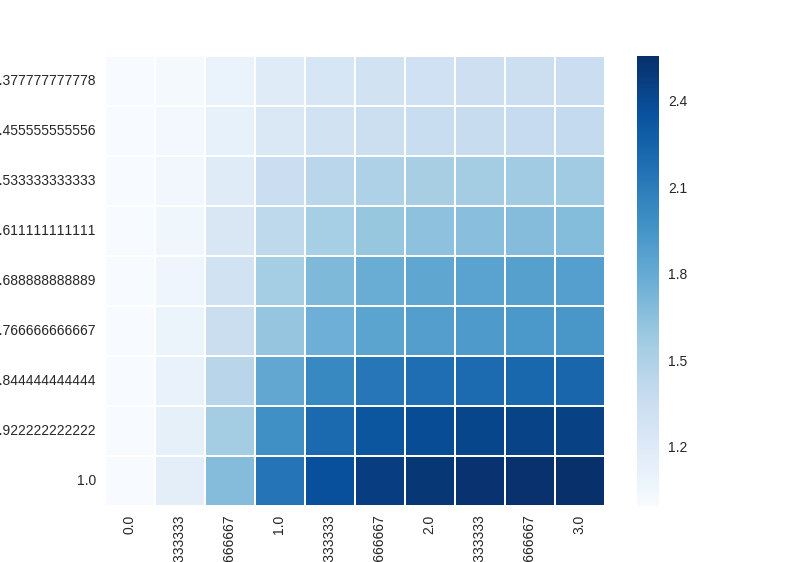
\includegraphics[scale=0.45]{l2fusionquick.png}
  \caption{\label{fig:figure1} We generate a series of networks with 20 TFs by 200 genes, with 75\% sparsity, 0.1 measurement noise, and 0.1 fusion noise. We hold lamP and lamR constant at 1.0 and 2.0 respectively. The x-axis represents lamS and the y-axis represents the proportion of nodes which are orthologous. As the networks increase in similarity, performance improves and benefits from a large fusion penalty weight. NOTE: This figure shows AUPR. $R^2$ behaves as expected with respect to $\lambda_S$ (networks with large differences between fused coefficients have best $R^2$ at intermediate $\lambda_S$). This doesn't really seem to be the case with AUPR. Maybe these early figures should be replaced with $R^2$}
  \end{center}
\end{figure}

\begin{figure}
\begin{center}
  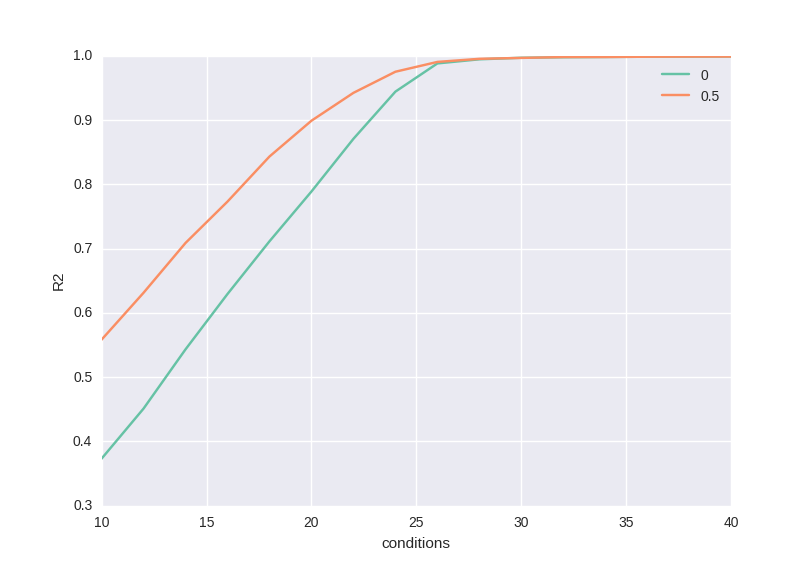
\includegraphics[scale=0.45]{increase_data2.png}
  \caption{\label{fig:figure1} We fuse two networks, both with 25 TFs by 50 genes, using lamS=0 and nonzero lamS, and hold the number of conditions in network 1 constant while varying the number of data points for network 2. We plot the performance of network 2.}
  \end{center}
\end{figure}

\subsection{Network similarity and fusion performance}
We assessed how varying the similarity of simulated networks affected network inference performance with fusion. The main factors governing similarity between our generated networks were the extent (and accuracy) of the orthology mapping, and the magnitude of variability between analogous interactions. We conducted a series of simulations to assess the effect of varying orthology coverage on networks in which analogous interactions varied little from one another. In order to determine the effect of the size of the orthology mapping on network inference performance, we simulated a series of 20 TFs by 200 genes networks at several values of percent orthology coverage. 

As expected, increasing the weight of the fusion constraint $\lambda_S$ improved network recovery (Figure 2). Networks with higher orthology coverage saw a greater benefit from fusion, although the improvement was not limited to analogous interactions. One way of assessing the effect of fusion on network inference performance is to compute an ``exchange-rate'' between conditions in each network. Suppose you are interested in determining a regulatory network for species A, a model organism which is experimentally inconvenient. A related species, B, is easier to collect data for, but of less intrinsic interest. Our simulation results suggest that adding conditions from species B to a fused network inference problem has an effect on network A recovery that is similar to adding conditions from A at a reduced rate (Figure 3). 

We also assessed the effect of varying the standard deviation of the distribution of differences between analogous interactions on network performance. FILL IN. MENTION PRIOR INTERPRETATION

\begin{figure}
\begin{center}
  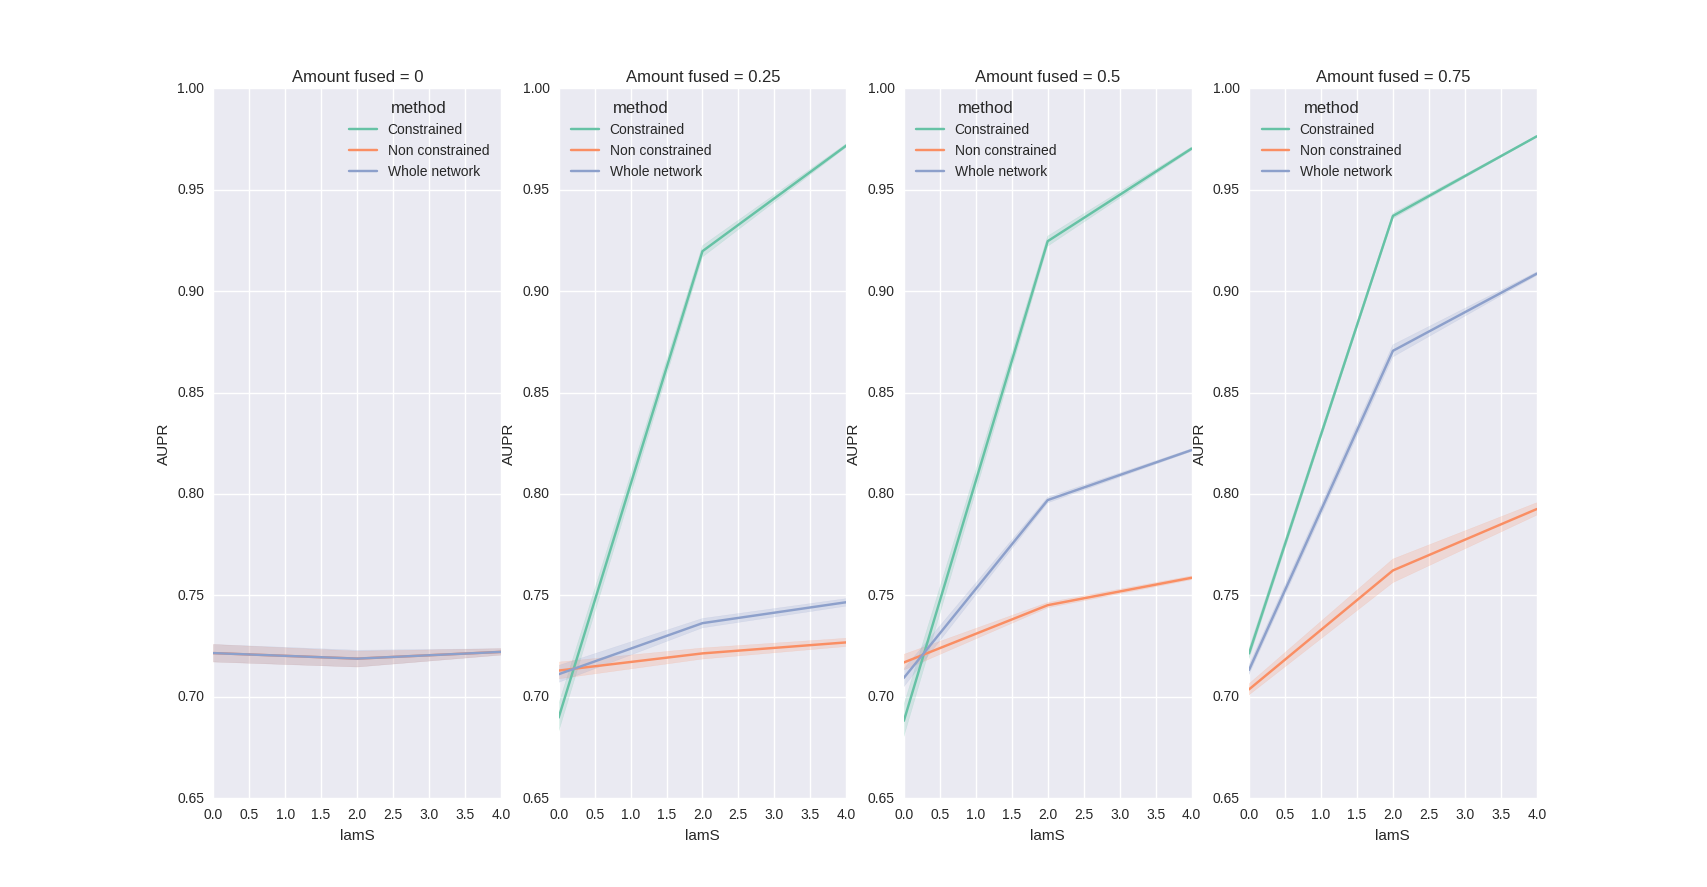
\includegraphics[scale=0.45]{con_noncon.png}
  \caption{\label{fig:figure4} We looked at four different sets of networks, each with 20 TFs by 200 genes, where each set had different amounts of orthologous genes. We plotted the performance on the whole network, the constrained, and non-constrained portions of the network as we increased the fusion penalty weight.}
  \end{center}
\end{figure}

\subsection{Fused regression improves performance on both the constrained and non-constrained parts of the network}
We wanted to know if using fused regression on networks with only conserved subgraphs affected the recovery of the non constrained parts of the networks (Figure 4). We used sets of two networks with 20 TFs and 200 genes each, where each set had 0\%, 25\%, 50\%, or 75\% of the TFs and genes in orthology groups. We varied lamS and computed AUPR using cross-validation on the portion of the network that had fusion constraints, the portion without any orthology information, and on the whole network. On the fused networks, performance improved as the fusion penalty weight increased; interestingly, performance gains were seen even the portion of the network where no orthology information is known. By constraining part of an underdetermined system, we obtained gains in both parts. 

\begin{figure}
\begin{center}
  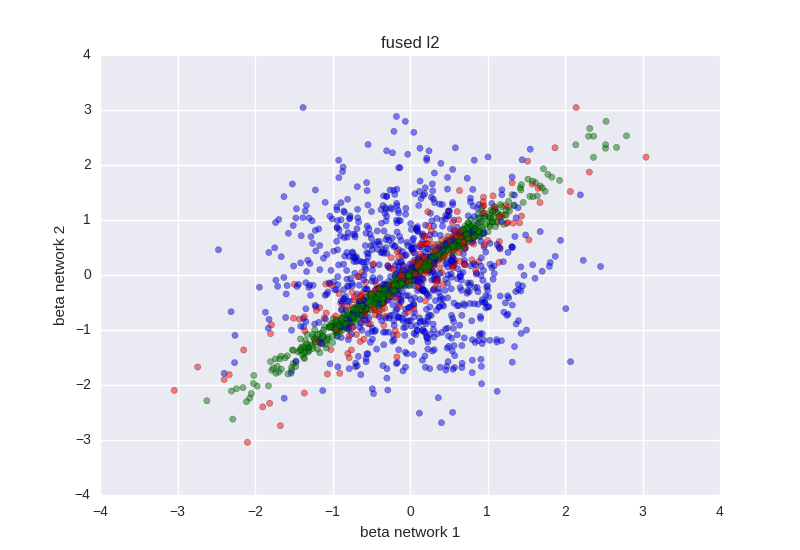
\includegraphics[scale=0.45]{plot_betas_scad_l2.png}
  \caption{\label{fig:figure1} We used two networks, each with 20 TFs by 200 genes, 50\% of which are orthologous. We include as many false positive orthologs as true positives, and color the points solved using true orthology information green and the points solved using false orthology information red. We randomly select an interaction from each network, and color this point blue. We solve the networks using fused L2.}
  \end{center}
\end{figure}

\begin{figure}
\begin{center}
  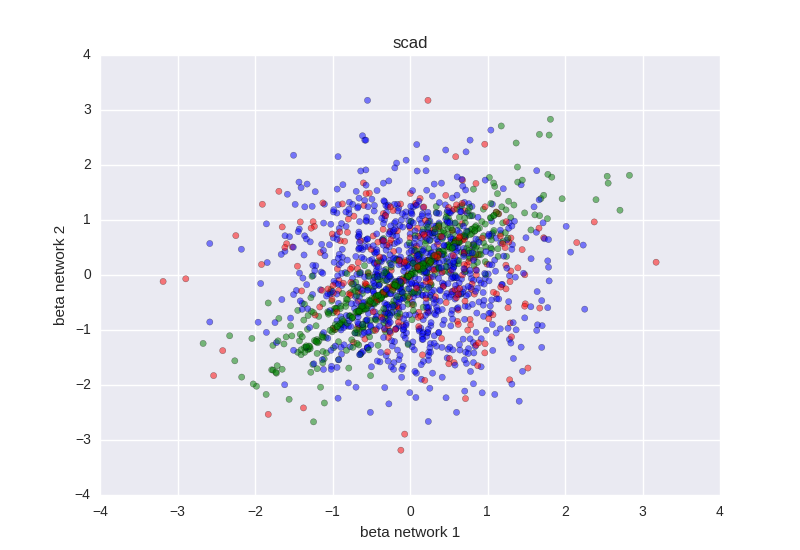
\includegraphics[scale=0.45]{plot_betas_scad.png}
  \caption{\label{fig:figure1} We used two networks, each with 20 TFs by 200 genes, 50\% of which are orthologous. We include as many false positive orthologs as true positives, and color the points solved using true orthology information green and the points solved using false orthology information red. We randomly select an interaction from each network, and color this point blue. We solve the networks using adaptive fusion.}
  \end{center}
\end{figure}

\begin{figure}
\begin{center}
  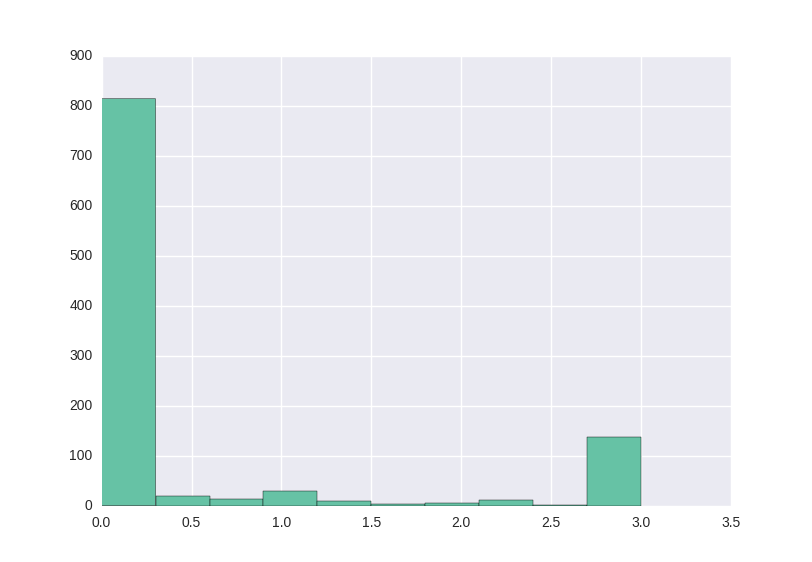
\includegraphics[scale=0.45]{scadf.png}
  \caption{\label{fig:figure1} Here we use two 10 TF by 200 gene networks, 50\% of which are orthologous. We include as many false positive orthologs as we have true positives, and apply adaptive fusion to the beta values with lamS=3. We plot the distribution of lamS learned for false orthologs.}
  \end{center}
\end{figure}

\begin{figure}
\begin{center}
  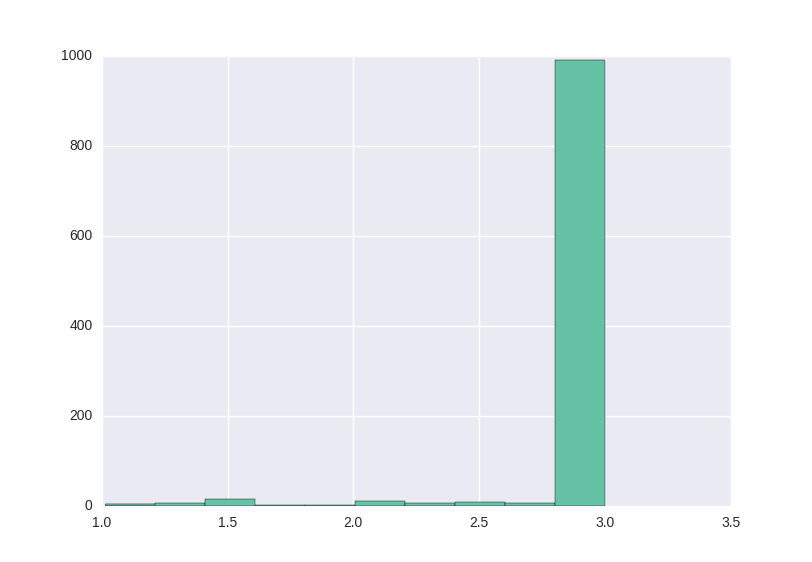
\includegraphics[scale=0.45]{scadt.png}
  \caption{\label{fig:figure1} Here we use two 10 TF by 200 gene networks, 50\% of which are orthologous. We include as many false positive orthologs as we have true positives, and apply adaptive fusion to the beta values with lamS=3. We plot the distribution of lamS learned for true orthologs.}
  \end{center}
\end{figure}

\subsection{Adaptive fusion successfully identifies and unfuses 'neofunctionalized' genes}
We recognize that orthology prediction is not necessarily a perfect proxy for functional conservation. We implemented an adaptive fusion algorithm that attempts to optimize a nonconvex saturating penalty function on differences between fused interactions. Pairs of interactions which are very dissimilar even after fusion, which sit in the flat portion of this penalty function, are effectively ``unfused''. We can interpret this ``unfusing'' as evidence for neofunctionalization of one or more of the genes involved in this pair of interactions. 

We performed a simulation to assess the ability of our adaptive fusion algorithm to learn which parts of two input networks are conserved when orthology information is faulty, to mimic orthologs which are not functionally analogous  (Figure 5-8). We generated synthetic fused networks and introduced error in the fusion constraints by adding false positives and negatives to the orthology information given to the solver. Because we knew which entries in the orthology mapping were ``fake'' (not reflected in the generation of the networks), we could correctly label fusion constraints that involved one or more ``fake'' mappings. We verified that adaptive-fusion unfused mostly ``fake'' interactions, while leaving truly analogous interactions fused.

\begin{figure}
\begin{center}
  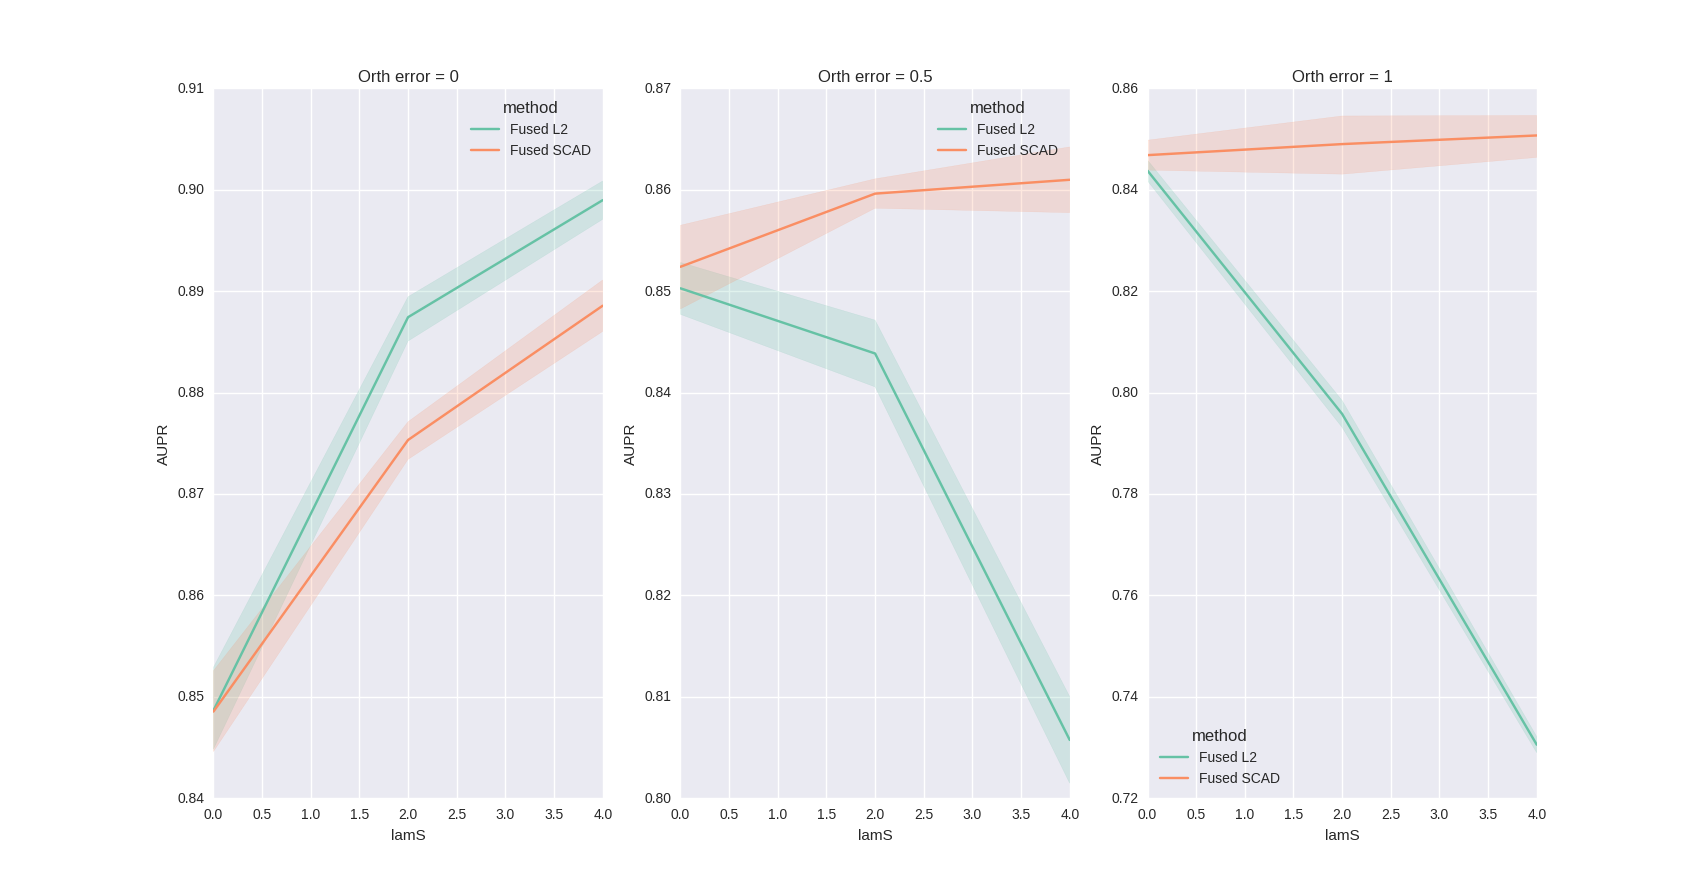
\includegraphics[scale=0.45]{test_scad_opt_params3.png}
  \caption{\label{fig:figure1} We use three sets of 20 TF by 200 gene networks, 50\% of which are orthologs, and solve with orthology information containing 0:1, 0.5:1, and 1:1 false positive to true positive. We plot AUPR under fused L2 and adaptive fusion.}
  \end{center}
\end{figure}

\subsection{Adaptive fusion improves network inference}
We wanted to determine whether adaptive fusion is able to improve learning of GRNs. That is, beyond correctly identifying functional conservation and recovering the performance lost by fusing neofunctionalized genes, is our method able to produce more accurate networks than those learned without fusion? (Figure 9) We again generated synthetic fused networks and added false positive and negative orthologs, then used fused L2 and adaptive fusion approaches to solve the underlying network. Fused L2 incorporated flawed orthology information, resulting in degradation of performance as we increased orthology error. Performance increased using adaptive fusion, pointing to its utility in network inference in addition to identifying neofunctionalization.


\section{Bacterial data}
We used gene-expression data from B. subtilis and B. anthracis in order to assess performance gains of fused regression on real data. Our B subtilis data set consists of 266 time-series and steady-state observations of 4891 genes during development. Our B. anthracis dataset consists of 72 time-series and steady-state observations of 5536 genes comprising data from developmental and iron-starvation conditions. There were 247 known Transcription Factors (TFs) in the B. subtilis dataset, and 248 TFs in the B. anthracis dataset. 

We obtained 1870 one-to-one orthologs from Inparanoid, which produced 177650 fusion-constraints between gene interactions within the two species. Although this number seems very large, it represents only $14.7\%$ of the regulatory interaction matrix in B. subtilis and $12.9\%$ in B. anthracis. The use of such dissimilar species is a test of whether fusion can improve network-inference even when the overlap in interactions is very small.

In order to evaluate network inference performance, and for use as priors, we used a gold standard of 2896 known B. subtilis interactions with corresponding activation and repression sign. Of these 2896 priors, 968 had corresponding interactions in B. anthracis. Based on our simulation results, we can expect the greatest gains in network-inference performance from fusion when the species of interest has a small number of available conditions, but data is abundant in a related species. However, in order to evaluate performance objectively a gold-standard of known interactions is necessary. As a result, we can only evaluate network recovery for B. subtilis, and B. subtilis also has the majority of our conditions. In order to simulate the data-poor regime, we subsampled our B. subtilis data. Specifically, we divided our B. subtilis data into $k$ folds, and then for each fold fit a network to the B. subtilis data from that fold alone fused to the entire 72 B. anthracis conditions. We can then compute performance metrics (ie AUPR) for each fold, and use their variability across folds to test for significance of any improvements relating to the use of fusion constraints. 

\subsection{Bacterial performance}
\subsubsection{Performance with priors}
We want to show that performance increases with introduction of priors - this is easy/circular but important to show that our method can effectively incorporate priors

\subsubsection{Adaptive fusion}
We want to show that we can successfully identify neofunctionalization; since we do not have a gold standard for this we will introduce false positive orthologs into the orthology information and evaluate the ability of our method to identify true from false orthologs. 

\subsubsection{Precision recall}
Introducing fusion constraints leads to a small but consistent improvement in AUPR. Inspection of precision recall curves shows that this improvement is a result of increased precision at low values of recall. Essentially, precision increases for the high confidence part of the network but not for the low confidence part of the network. As a result, the improvements in performance may be more useful than would be suggested by AUPR alone. Interactions suggested by genome wide analysis need to be experimentally verified, and the ranking of interactions produced by a network inference algorithms is a useful guide to what order these experiments should be carried out in. The high confidence part of the network represents interactions that are likely candidates for experimental validation, so improvement in recovery of these interactions is particularly useful in guiding research. 


\begin{center}
  \begin{tabular}{ l | l | l }
    \hline
    $\lambda_S$ & $\%$ data & $AUPR constrained$ \\ \hline
    0 & 0.066 & 0.0390 \\
    5 & 0.066 & 0.0415 \\
    \hline
  \end{tabular}
\end{center}


\begin{figure}
\begin{center}
  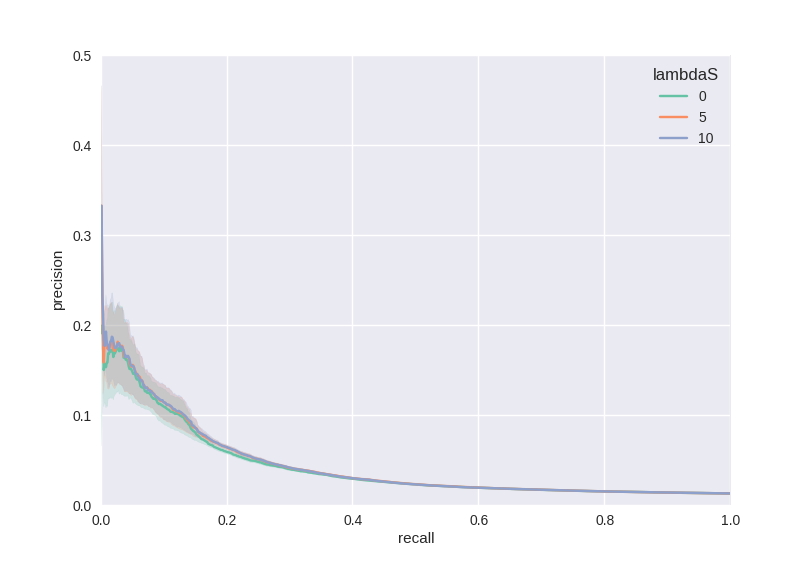
\includegraphics[scale=0.45]{waka7unnormed.png}
  \caption{\label{fig:figure1} precision recall curves of constrained interactions for several values of lamS, computed across folds containing $\frac{1}{15}th$ of the available B. Subtilis data}
  \end{center}
\end{figure}

\begin{figure}
\begin{center}
  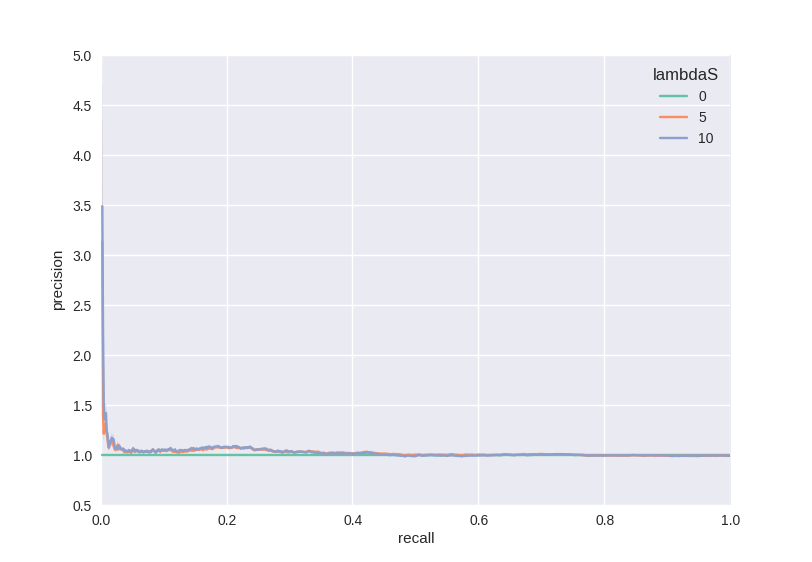
\includegraphics[scale=0.45]{woko7.png}
  \caption{\label{fig:figure1} normalized precision recall curves of constrained interactions for several values of lamS, computed across folds containing $\frac{1}{15}th$ of the available B. Subtilis data. Normalization involved dividing the precision each each recall level, for each curve, and for each cross-validation fold by the corresponding $\lambda_S=0$ precision.}
  \end{center}
\end{figure}

\begin{figure}
\begin{center}
  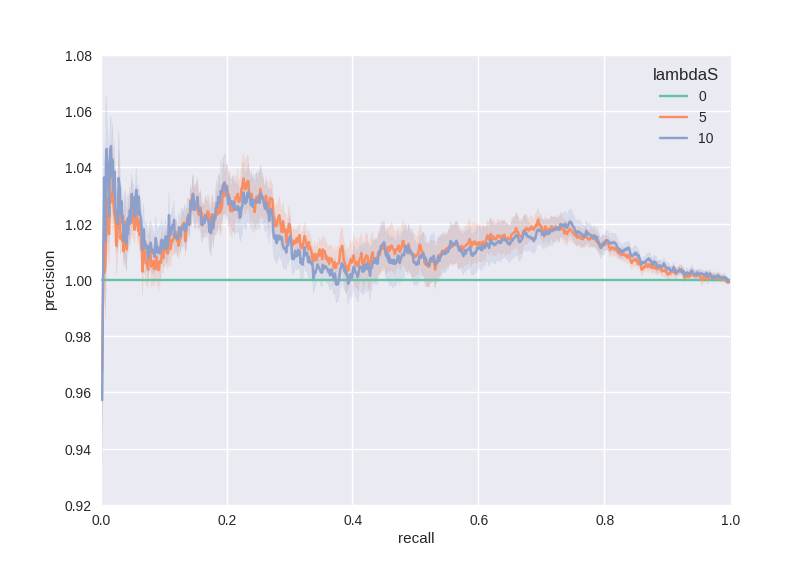
\includegraphics[scale=0.45]{wat7.png}
  \caption{\label{fig:figure1} As previous figure, but for all interactions.}
  \end{center}
\end{figure}


\bibliographystyle{plain}
\bibliography{paper}

\end{document}


